% !TEX root = main.tex

\paragraph{RQ1: Is spontaneous eye blink rate related to performance or Flow?}

sEBR showed a negative relationship to participant-wise LC slopes, as shown in Fig.~\ref{fig:EBRvLC}. The correlation is of moderate strength, though non-significant (Pearson's {\it r} = -.46 , {\it p} = 1.0, N = 9). %NHST13
The LC slope of every participant was negative, which means we can say that the smaller the sEBR, the shallower the LC slope. Or, because slope and intercept are highly correlated, it is almost equivalent to say that smaller sEBR correlates with better initial performance.

Mean Flow scores are not related to sEBR, as can be seen in Fig.~\ref{fig:EBRvLC} (Pearson's {\it r} = 0.15, {\it p} = 1.0, N = 9). %NHST14
However, examining the Flow scores in Fig.~\ref{fig:EBRvLC} turns up an interesting relationship: the residuals of the fitted linear model (i.e. vertical distance of each data-point from the line) are {\it strongly} related to mean Flow scores (Pearson's {\it r} = -.86 , {\it p} = .04, N = 9). %NHST15
In other words, participants' mean Flow scores are strongly correlated with their observed deviation from the modelled linear relationship between sEBR and task learning (LC slope). This correlation is not driven only by the non-significant correlation of Flow and LC (described above). In fact, interaction analysis (see Table~\ref{tab:simpslopes}) shows that when Flow mean is above 5.05, LC slope significantly predicts sEBR at {\it p} $<$ 0.0001.
%%%% FLOW X SEBR COR TEST
% data:  FM and sEBR
% t = 0.41014, df = 7, p-value = 0.694
% alternative hypothesis: true correlation is not equal to 0
% 95 percent confidence interval:
%  -0.5688016  0.7418380
% sample estimates:
%      cor
% 0.153187

%%%% FLOW X RESIDUAL COR TEST
% data:  FM and abs(LC - LM$fitted.values)
% t = -4.4556, df = 7, p-value = 0.002952
% alternative hypothesis: true correlation is not equal to 0
% 95 percent confidence interval:
%  -0.9700331 -0.4562393
% sample estimates:
%       cor
\begin{figure*}[!ht]
	\centering
	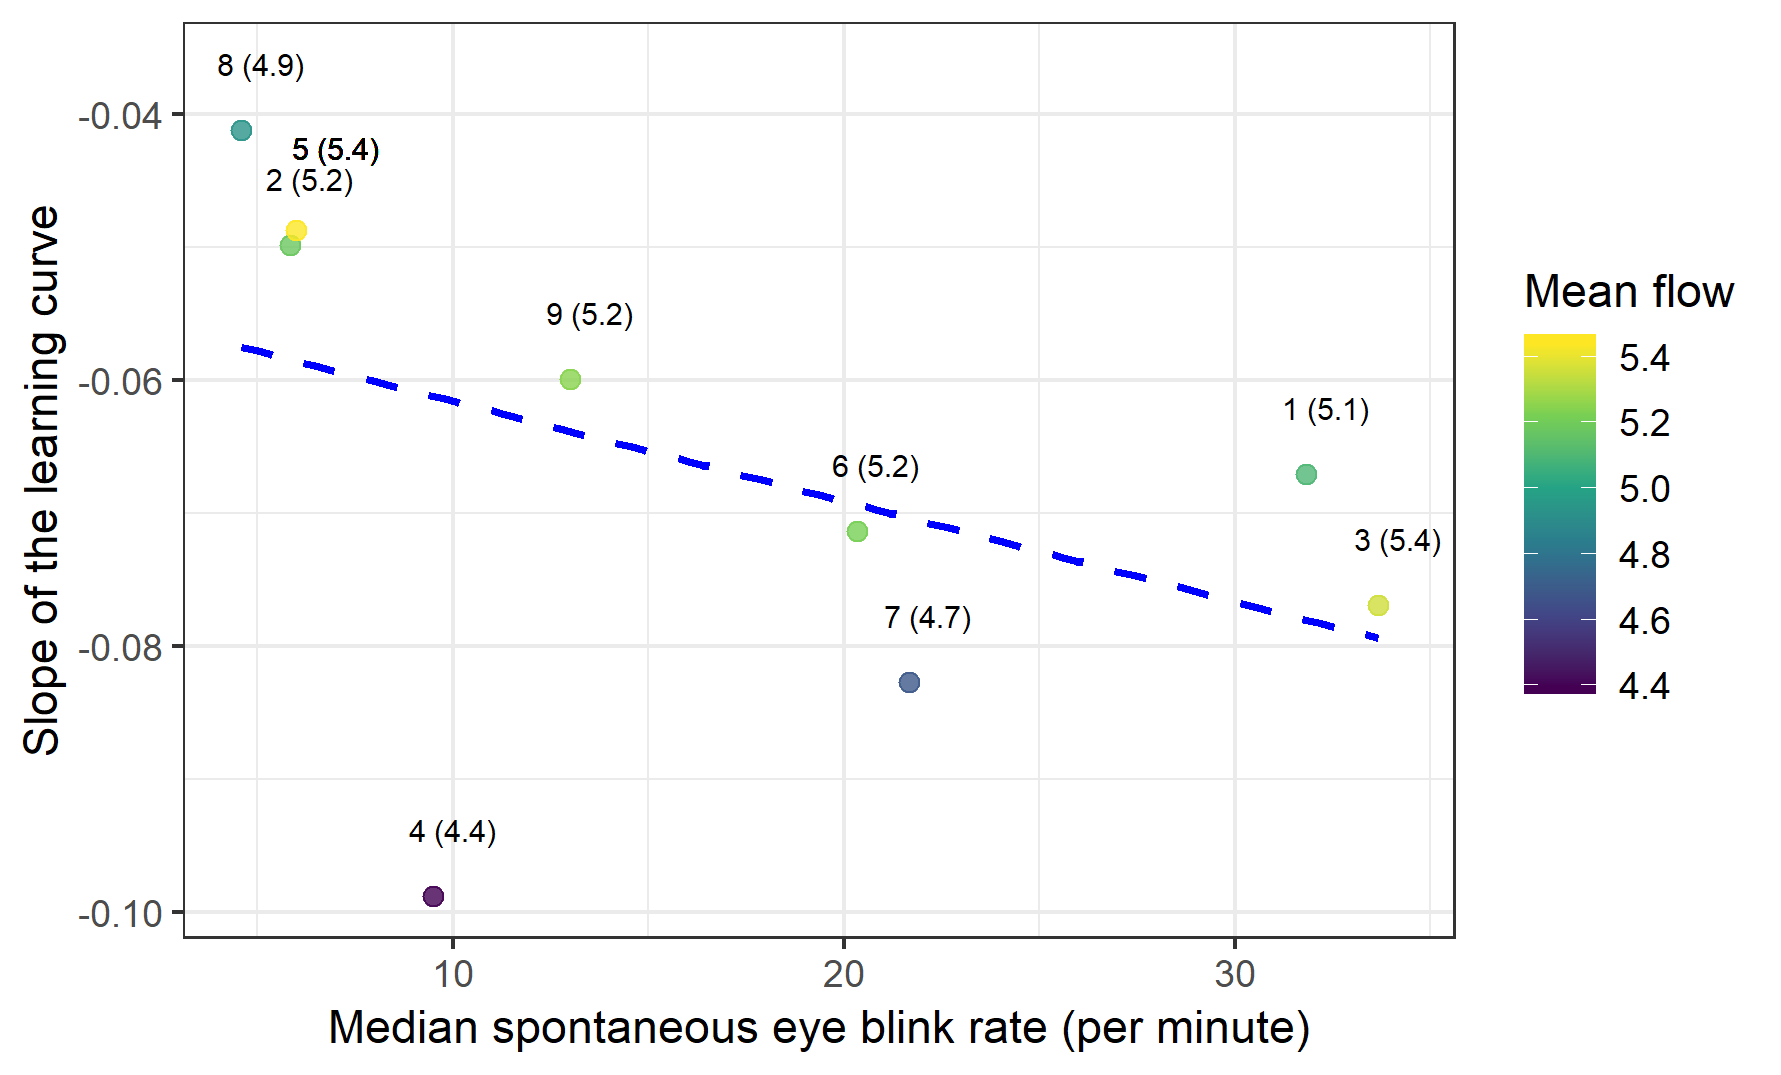
\includegraphics[width=\nicewidth]{lcurve_sbr_flowRL2}
	\caption{Participants' median spontaneous eye blink rate plotted against the slope of their learning curve, and coloured by their mean Flow scores. Linear model is depicted by the dashed line. Each point is labelled with the participant number (1..9) and exact mean Flow score (in parentheses).}
	\label{fig:EBRvLC}
\end{figure*}


% -0.859833

\begin{table}[!hb]
\centering
\caption{Outcome of simple-slopes analysis for Flow$\times$LC interaction: each row reports on the slope of LC slope at the level and value of Flow shown.}
\begin{tabular}{llllll}
\hline
Flow level & Flow & Est. & S.E. & t value & p \\
\hline
+ 1 SD & 5.40 & -1096.31 & 221.36 & -4.95 & 0.0002 \\
Mean   & 5.06 &  -683.33 & 143.15 & -4.77 & 0.0002 \\
- 1 SD & 4.73 &  -270.35 & 158.23 & -1.71 & 1.0 \\
\hline
\label{tab:simpslopes}
\end{tabular}
\end{table}

% SIMPLE SLOPES ANALYSIS
% Slope of LC when FM = 5.40 (+ 1 SD):
%      Est.   S.E. t val.    p
%  -1096.31 221.36  -4.95 0.00
% Slope of LC when FM = 5.06 (Mean):
%     Est.   S.E. t val.    p
%  -683.33 143.15  -4.77 0.00
% Slope of LC when FM = 4.73 (- 1 SD):
%     Est.   S.E. t val.    p
%  -270.35 158.23  -1.71 0.15
%
%  JOHNSON-NEYMAN INTERVAL

\subsection*{RQ2: blink rate and Flow components}
{\it session-wise within-subjects}
